\chapter{Controlled Nuisance Sensitivity and Reference Calibration}\label{chap:synthetic}
\label{ch:synthetic}

This chapter reports what the matched synthetic studies establish about detecting marked stress sensitivity when parts of the background and triggering process are estimated. The historical comparisons below concern their stated law class and finite numerical implementation; the subsequent F continuation is reported separately at the end of the chapter. The common alternative bank contains \(150\) stronger histories, and each procedure has \(1{,}000\) null queries with \(999\) separately identified null references. Success is a calibrated rejection on an alternative history; the null rejection rate counts rejections among uninhibited query histories. Figure~\ref{fig:detection} summarizes the detection rates and their conditional binomial intervals.

\begin{table}[tbp]
\centering
\caption{Historical detection on the common stronger alternative bank and null rejection on \(1{,}000\) null queries. Intervals are nominal \(95\%\) Clopper--Pearson intervals conditional on the fixed bank and law.}
\label{tab:main-detection}
\small
\setlength{\tabcolsep}{4pt}
\begin{tabular}{@{}p{0.40\linewidth}ccc@{}}
\toprule
Procedure & Detections & \(95\%\) interval & Null rejections \\
\midrule
Known laws (fixed \(\eta\)) & \(150/150\) & \(97.57\)--\(100\%\) & \(50/1000\) \\
\(\eta\) estimated; nuisances supplied & \(150/150\) & \(97.57\)--\(100\%\) & \(49/1000\) \\
Level estimated; trend supplied & \(123/150\) & \(74.90\)--\(87.79\%\) & \(46/1000\) \\
Level and trend estimated & \(68/150\) & \(37.20\)--\(53.66\%\) & \(44/1000\) \\
Historical fuller fitted procedure & \(57/150\) & \(30.21\)--\(46.28\%\) & \(50/1000\) \\
\bottomrule
\end{tabular}
\end{table}

For the first four procedures, the triggering process, mark exponent \(\beta\), and both kernels are supplied. The first row supplies both laws completely. The second estimates \(\eta\) while supplying the remaining nuisance values. The third estimates \(\eta\) and background level while supplying the trend, and the fourth estimates \(\eta\), background level and trend. The final row is the fuller historical fitted procedure, which additionally estimates or searches the triggering, mark, and kernel components under the earlier recipe. It is therefore not a purely nested extension of the fourth row, and its count should not be interpreted as an independent replication.

The known-laws (fixed \(\eta\)) procedure detects every one of the \(150\) stronger alternatives. This demonstrates that, for the evaluated generating law and numerical kernels, the stronger marked sensitivity is distinguishable when the comparison laws are supplied. It is not a statement of intrinsic inability to distinguish arbitrary physical mechanisms, nor a proof that all mechanisms would be easy to distinguish in observed data. The \(\eta\)-estimated, nuisances-supplied procedure also detects all \(150\). There is no observed loss from estimating that parameter alone on this bank; this does not prove equality of population detection probabilities. Estimating the background level leaves \(123\) detections, while estimating both level and trend leaves \(68\). These named-procedure differences are not an additive attribution of the gap. Moving from \(150\) to \(123\) and from \(123\) to \(68\) describes the tested configurations; it does not decompose the loss into independently estimable physical or numerical contributions.

The realized null rates lie between \(4.4\%\) and \(5.0\%\). In row order, the conditional \(95\%\) null intervals are \(3.73\)--\(6.54\%\), \(3.65\)--\(6.43\%\), \(3.39\)--\(6.09\%\), \(3.21\)--\(5.86\%\), and \(3.73\)--\(6.54\%\). These similar observed rates are useful calibration summaries, but they do not establish equal test size uniformly over the composite null. The intervals are conditional on the realized reference bank and law, and the procedures were selected through research reuse.


\begin{figure}[tbp]
\centering
\includegraphics[width=\linewidth]{detection.pdf}
\caption{Historical matched-null detection on the same 150 stronger alternatives. Error bars are nominal conditional 95\% binomial intervals. Each procedure has its own 999 reference statistics and 1,000 separate null queries; adaptive selection and reference-bank uncertainty are omitted.}
\label{fig:detection}
\end{figure}

\section{Sensitivity to the diagnostic value}

The value of \(\eta\) changes the histories as well as the fixed-history intensity separation. In a paired comparison using the same \(150\) fresh pairs, the initial value \(\eta=0.2839974288868791\) produced \(49/150\) detections for the fuller fitted procedure, whereas the adjusted value \(\eta=0.4885010300470942\) produced \(57/150\). The paired gain is therefore \(8\) detected histories, or \(5.33\) percentage points, with a descriptive Monte Carlo standard error of \(4.71\) percentage points. A separate \(25\)-pair planning sample gave \(6/25\) and \(11/25\) under the two values; it is a planning exercise and is not pooled with the \(150\)-pair comparison.

The descriptive paired Monte Carlo standard error uses the sample variance of paired decision differences. For \(N_{\mathrm{pair}}\) pairs, let \(D_i\in\{-1,0,1\}\) be the first decision minus the second, with positive and negative discordance counts \(b,c\). Then
\[
 \overline D=\frac{b-c}{N_{\mathrm{pair}}},\qquad
 \widehat{\operatorname{MCSE}}
 =\sqrt{\frac{b+c-N_{\mathrm{pair}}\overline D^{\,2}}
 {N_{\mathrm{pair}}(N_{\mathrm{pair}}-1)}}.
\]
This is the sample standard deviation of \(D_i\) divided by \(\sqrt{N_{\mathrm{pair}}}\). Taking the adjusted-value decision first gives \(b=29,c=21\) and \(N_{\mathrm{pair}}=150\), hence \(4.7096\) percentage points, rounding to \(4.71\). Using empirical-variance divisor \(N_{\mathrm{pair}}\) instead gives a slightly different value from the same outcomes. The stated fixed-bank and adaptive-reuse qualifications still apply; no new test is added.

The mean achieved fixed-history total intensity suppression was \(14.159\%\) for the initial value and \(19.360\%\) for the adjusted value. For a realized nonempty history and fixed generating nuisance, the event-mean functional is
\begin{equation}
 S(\eta;\mathcal H_T)=\frac{100}{N_T}\sum_{i=1}^{N_T}
 \frac{B(t_i)\{1-e^{-\eta G_s(t_i)}\}}
      {B(t_i)+nH_e(t_i)}.
 \label{eq:achieved-suppression}
\end{equation}
Both intensities in each comparison use the same strictly earlier history. The reported mean then gives equal weight to each catalogue's event mean, rather than pooling every event across catalogues. This is the functional implemented in \hyperlink{S07}{archival \texttt{S07} (not distributed)}.
It is an event-mean description of separation on a common history, not a controlled reduction in earthquake count. Increasing \(\eta\) also changes the synthetic histories that are subsequently realized. Counts remain random, and no monotonicity of realized counts is guaranteed. An extreme retained pair, with \(449\) events under one member and \(6{,}553\) under the other, illustrates why suppression of a fixed-history rate cannot be reported as a promise about realized totals.

An earlier archive used a \(1{,}999\)-reference rank denominator of \(2{,}000\). The later recalibration using \(999\) references and \(1{,}000\) separate null queries produced the same count of \(57\) detections only by happenstance. It is a consistency observation, not an independent replication, and the two reference constructions should not be combined. The \href{https://github.com/Drefetr/InhibitoryEarthquakeModels/blob/3e76a174cf4f58ce601c6c9640c4d0c11168813f/paper/data/paired.json}{public paired summary} retains aggregate pairing results; the historical study is reported in \hyperlink{S08}{archival \texttt{S08} (not distributed)}. The completed-history provenance for later recalibration is recorded in \hyperlink{S09}{archival \texttt{S09} (not distributed)} and the final results in \hyperlink{S16}{archival \texttt{S16} (not distributed)}.

\section{Paired comparison of level and trend}

The level-and-trend comparison is more informative when the two procedures are paired on the same \(150\) histories rather than read only from marginal detection counts. Figure~\ref{fig:paired} crosses their decisions. Both procedures detect on \(62\) histories, the level-only procedure detects on \(61\) where the combined procedure does not, the combined procedure detects on \(6\) where level-only does not, and neither detects on \(21\). The marginal counts are therefore \(123\) and \(68\), and the difference is \(55/150=36.67\) percentage points, with a descriptive paired Monte Carlo standard error of \(4.58\) percentage points, using the same sample-variance convention with \(b=61,c=6\) and \(N_{\mathrm{pair}}=150\) (\(4.5776\) before rounding).

There is no pathwise dominance. The level-only procedure detects on \(61\) histories where the combined procedure does not, while the reverse occurs on \(6\). The \(55\)-history marginal gap is real for this realized paired bank, but the paired arrangement shows that it is not produced by a uniform improvement. Among the \(999\) null reference scores for the level-only procedure, \(604\) were exactly zero. Ties and the add-one rank rule are therefore material in that calibration. Different null thresholds can alter the comparison and must be considered when interpreting the paired decisions.

A ten-history raw-statistic pilot contained six null and four alternative histories. On that small pilot, level-only contraction exceeded trend-only contraction on four alternatives. This is a descriptive diagnostic of local score behavior, not a calibrated power comparison. That historical experiment does not contain a fully calibrated trend-only row, so the level-only discordance cannot be assigned uniquely to trend. The absence of that row does not imply that trend-only would perform best, nor does it automatically identify trend-only calibration as the best next experiment. A fair decision among procedures would require its own reference bank and calibration under the same reporting rules.

All \(1{,}150\) decisions in the reported historical detection-and-null evaluation resolved under the empirical numerical envelopes. That is a completeness statement for this realized study, not a rigorous universal bound on numerical integration or optimization. The selected-ten pilot is documented in \hyperlink{S15}{archival \texttt{S15} (not distributed)}. The paired detection table and matched-null results are documented in \hyperlink{S16}{archival \texttt{S16} (not distributed)}.


\begin{figure}[!htbp]
\centering
\includegraphics[width=0.68\linewidth]{paired.pdf}
\caption{Paired decisions for background level alone versus level and trend estimated. The 61 versus six discordant histories yield a 36.67 percentage-point net difference, but neither procedure dominates on every history.}
\label{fig:paired}
\end{figure}

\section{Diagnostics and limits of explanation}

A separate audit examined ten selected difficult completed histories using a larger iteration limit and a Powell search. The largest phase improvement in negative log likelihood was \(1.94995664\times10^{-8}\), and the largest direct generalized-likelihood-ratio change was \(3.89681745\times10^{-8}\), below the declared diagnostic screens of \(0.001\) for phase negative log likelihood and \(0.1\) for the direct statistic. These histories were selected because they were difficult, so the audit is neither representative of the full bank nor a global optimization guarantee. Within the audited set, however, it weakens an explanation of the fitted-law gap based on inadequate optimizer stopping. It does not eliminate the possibility of optimizer limitations on other histories. This selected-ten audit concerns the historical recipe; the later F solver diagnostics and unresolved outcomes are separately reported in the addendum.

Two pre-existing fixed-history score projections onto \(a\), \(d\), and \(n\) retain \(10.82\%\) and \(3.26\%\) of weighted \(\eta\) squared-score norms. These percentages show local overlap between the directions in which the background parameters and the diagnostic parameter move the score. They are not ensemble Fisher information, not fractions of statistical power, and not an explanation of the observed \(38\%\) fitted detection rate.

Saved likelihood accounting provides one further descriptive check: estimating background level and trend improved the selected null likelihood more than the alternative likelihood on all \(150\) histories, with median null negative-log-likelihood gain \(28.665\) versus \(0.862\) for the alternatives. This records how the supplied comparison accounted for background in these specific histories. It is not a measurement of physical loading. The optimizer audit is reported in \hyperlink{S14}{archival \texttt{S14} (not distributed)}; the score geometry is reported in \hyperlink{S02}{archival \texttt{S02} (not distributed)}; and the saved likelihood accounting is documented in \hyperlink{S11}{archival \texttt{S11} (not distributed)}.

Taken together, the matched studies locate a substantial change in calibrated detection when background parameters are estimated: under the stated synthetic law, the stronger alternatives are distinguishable with supplied laws and with \(\eta\) alone estimated, while fitting background components changes the calibrated detection outcome. The experiments cannot separate the unavoidable difficulty of a composite statistical problem from recoverable loss in a particular fitted procedure. They are controlled matched-law tests rather than empirical physical discovery, and the reported boundaries follow from that design. The scoped contribution is a reproducible, numerically explicit assessment of where the marked-sensitivity signal is retained or attenuated by estimation, together with the calibration limits needed to read it. 

The \href{https://github.com/Drefetr/InhibitoryEarthquakeModels/blob/3e76a174cf4f58ce601c6c9640c4d0c11168813f/paper/data/detection.json}{public detection summary} and the \hyperref[sec:source-supplements]{availability guide} provide public entry points. Raw histories, role/seed/clock mappings and the complete executed known-law replay are supplied in \path{reproduction/synthetic/} and \path{reproduction/oracle/}. Available later fitted states are retained alongside those histories; the reproduction guide identifies the original restricted-fit states that remain missing.


% Let the completed historical discussion flow into the continuation.
\section{Background nuisance estimation: the four-procedure continuation}
\label{sec:f-continuation}\label{sec:f-continuation-full}
Scientific execution occurred on 19 October 2026 UTC (20 October in New Zealand at completion); the source editorial revision was dated 22 October 2026. No new scientific computation accompanies this consolidation.


This continuation reuses pinned historical input and clock identities but
applies its separately frozen finite solver and control recipe. Its trend-only
cell does not retrospectively explain the historical level-only discordance.
The historical counts, conditional intervals and figures above retain their
own recipes and are not pooled with or overwritten by this continuation.
The full matrix below replaces the former brief continuation summary.

The question is whether background nuisance treatment changes a fixed finite
inhibition procedure, and whether conditional likelihood compensation or
numerical stopping sensitivity helps explain the observed differences.
No physical or causal explanation follows merely from a favourable contrast.
All alternatives estimate inhibition $\eta$; the null fixes $\eta=0$.
\begin{center}
\begin{tabular}{lll}\toprule
Cell & Free null coordinates & Free alternative coordinates\\\midrule
$I_{00}$ & none & $\eta$\\
$I_{10}$ & $a$ & $(a,\eta)$\\
$I_{01}$ & $d$ & $(d,\eta)$\\
$I_{11}$ & $(a,d)$ & $(a,d,\eta)$\\\bottomrule
\end{tabular}
\end{center}
Here $a,d$ are background log level and trend; other parameters are supplied
according to the pinned law. Supplied/supplied is not a fixed-$\eta$ oracle.
The original procedure is distinct from the separately labelled solver
and geometry diagnostics.

\section{Strict marked-history accounting}
For a fixed observed history, write
\[
 \lambda(t)=\exp\{a+d x_{\mathrm{trend}}(t)-\eta G(t)\}+nH(t),\qquad
 \ell=\sum_i\log\lambda(t_i^-)+\sum_i\log f_\beta(q_i)
       -\int_0^T\lambda(t)\,dt .
\]
Here $x_{\mathrm{trend}}(t)=2t/(24394\,\mathrm{days})-1$ is the actual affine
observation coordinate, with $t$ measured in days; it is not $1/t$ or a
Taylor approximation.
Only earlier events enter $G(t_i^-),H(t_i^-)$. The current mark affects later
history, not its own event intensity. Initial quiet and terminal exposure,
all earlier parents and the exact supplied projected/paired clock convention
are retained. No clock or mark repair is introduced.

The direct contrast retains event and complete compensator accounting.
With the same supplied $n$, trigger kernel/productivity and mark law, trigger
exposure and common mark terms cancel between null and alternative. This is
an explicit cancellation, not a reason to omit those terms in comparisons
that change them. Event-log terms cannot be additively allocated to latent
causes. The primary numerical procedure is order 16 with mandatory order-32
and other prescribed controls. A finite candidate does not override an
unresolved optimizer or control status. Bounded recipes establish neither
global optima nor equal effective complexity.

\section{Conditional amplitude computation}
The conditional objective and its convexity in $A=e^a$, rather than in $a$, are derived once in Proposition~\ref{prop:amplitude} and equation~\eqref{eq:amplitude-objective}. The continuation uses that result with background integral $\mathcal B=\int_0^T e^{d x_{\mathrm{trend}}(t)-\eta G(t)}dt$ and fixed triggering contributions $v_i=nH_i$.
The constrained profile has $A\in[e^{-12},1]$. A nonnegative derivative at the lower endpoint selects that endpoint; a nonpositive derivative at the upper endpoint selects the upper endpoint; otherwise a bracketed scalar root is used. When all $v_i=0$, the unconstrained solution $N/\mathcal B$ is restricted to the allowed interval; an empty history selects the lower endpoint.

The implementation reports actual derivative/KKT tolerance, amplitude
bracket width, stopping reason and exact/approximate status. Its parameter
named \texttt{a\_tolerance} gates width in $A$, not absolute error in $a$.
Interior acceptance can be curvature/bracket-width limited; it must not be
described as meeting a fixed derivative threshold alone. The conditional
mesh fixes the remaining parameters and is not a confidence region.
The $\eta=0$ analytic background branch and positive-$\eta$ quadrature branch
have a separately recorded numerical seam. All four prescribed difference
steps are retained, with truncation/cancellation and boundary-domain cautions;
no best step repairs a scientific acceptance rule.

\section{Realized-event geometry}
At a fixed point the event log-intensity columns are
\[
 c_i=(p_i,\;p_i x_{\mathrm{trend}}(T_i),\;-p_iG_i),\qquad
 Z=W^{1/2}C_{\rm event} .
\]
Main06 uses $W=I_N$, so every actual event weight is one. The factors
$p_i$ already enter the event columns; quadrature weights are separate.
The raw Gram matrix is $Z^\top Z$. Nonzero weighted columns are normalized
by their Euclidean norms before numerical SVD/projection. If $\widetilde z_\eta$
is the scaled inhibition column and $P_{a,d}$ the numerical least-squares
projection on the scaled nuisance columns, the reported residual is
\[
 r_\eta=\frac{\|(I-P_{a,d})\widetilde z_\eta\|_2^2}
                  {\|\widetilde z_\eta\|_2^2} .
\]
This is a \emph{squared} residual fraction, not a norm ratio. A zero
inhibition column is explicitly undefined for interpretation, despite its
reported zero convention. The event Gram excludes compensator derivatives
and random-history variation: it is not a full observed Hessian, ensemble
Fisher information, sampling covariance, global identification theorem or
causal quantity. Low residuals describe conditional path overlap only.

\section{Historical incomplete checkpoint and its recovery}
The following accounting describes the earlier interrupted checkpoint. The completed recovery is reported at the end of this chapter.
The independently reviewed historical geometry stage was partial: six of 11 cases
completed, two timed out, one was started-unknown at the tree-RSS stop and
two were unattempted. All 11 remain in the accounting. The original figure displayed six completed meshes; the updated figure below includes the subsequently recovered profiles. At that checkpoint, the absent meshes are new\_r076 and null0945 (partial), null1292 (started-unknown), and null1322 and null1434 (unattempted). The saved
portion has 253 of 396 solver rows and 840 of 1,540 profile points, with
840 corresponding order-32 controls. Two old failure witnesses were
intentionally selected separately from nine metadata extrema; neither
selection estimates population prevalence or detection probability.

The old witnesses reproduced maxls=40 ABNORMAL returns; diagnostic
maxls=100 returned success at unchanged objective and essentially unchanged
parameters. This is stopping-flag sensitivity, not proof of the precise old
cause, gradient convergence or a corrected production outcome. No old
unresolved status is promoted, and maxls=100 is not substituted into calibration.

The separate ended nine-case full-procedure tail run produced seven complete
cases and 31 of 36 controlled method outcomes. One finite candidate lacked
final controls and four methods were absent; all five remain unknown.
The large alternative case timed out during its Powell control, while the
largest null case failed the unchanged internal 128 MiB feature-cache limit.
An external 2 GiB tree lease did not relax that internal limit or repair the
saved failure. These stress cases do not demonstrate complete bank coverage.

\begin{figure}[p]
\centering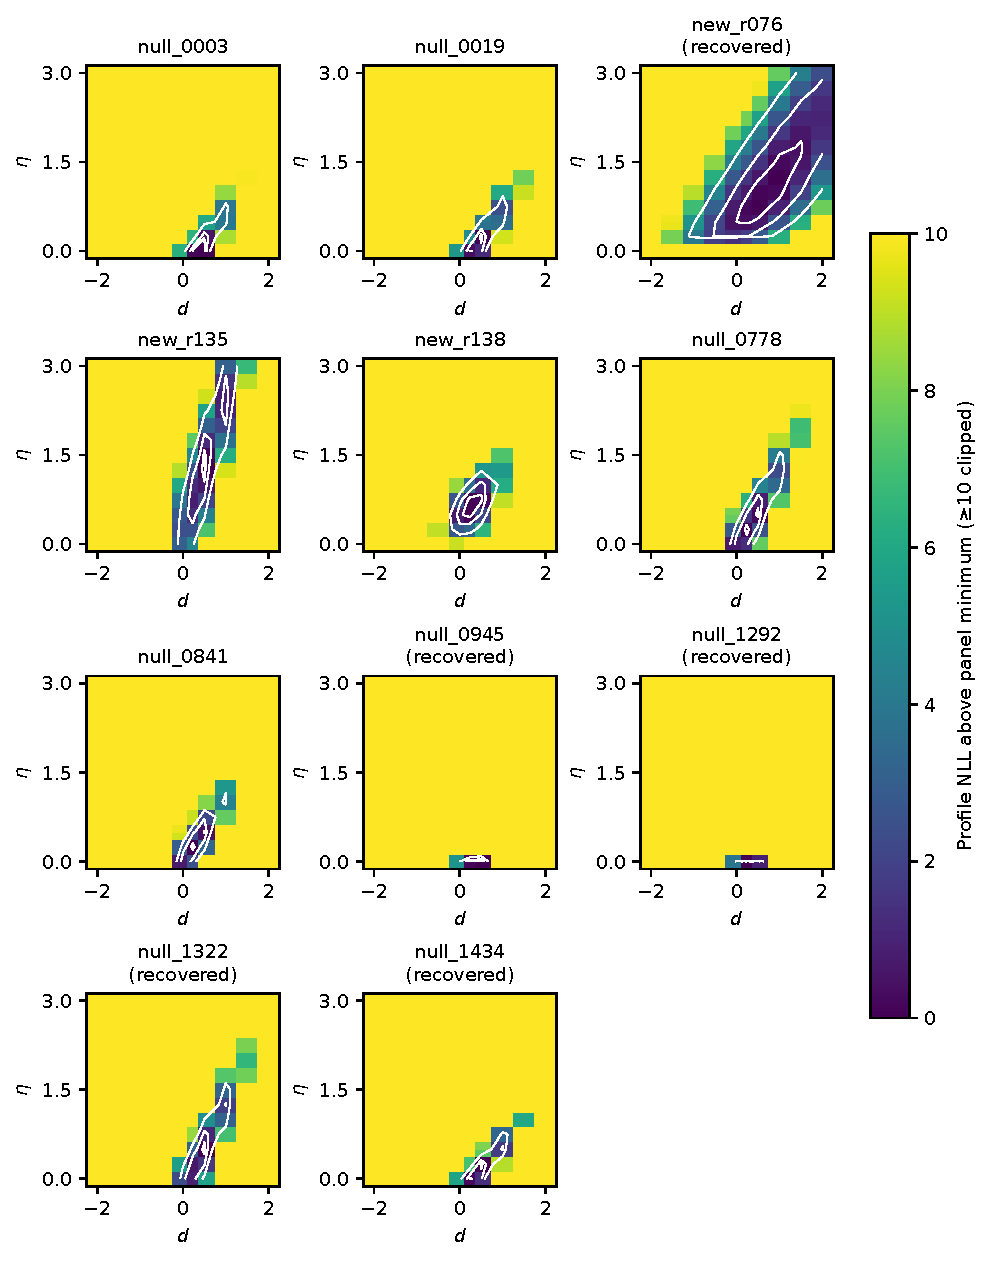
\includegraphics[width=\linewidth,height=.80\textheight,keepaspectratio]{s01_all11_profile_meshes.pdf}
\caption{Completed profile mesh cohort, with recovered panels marked. Each panel subtracts its own grid minimum; colour saturation is labelled. Completing profiles does not complete the historical Hessian diagnostics or establish a global optimum.}
\end{figure}
\begin{figure}[p]
\centering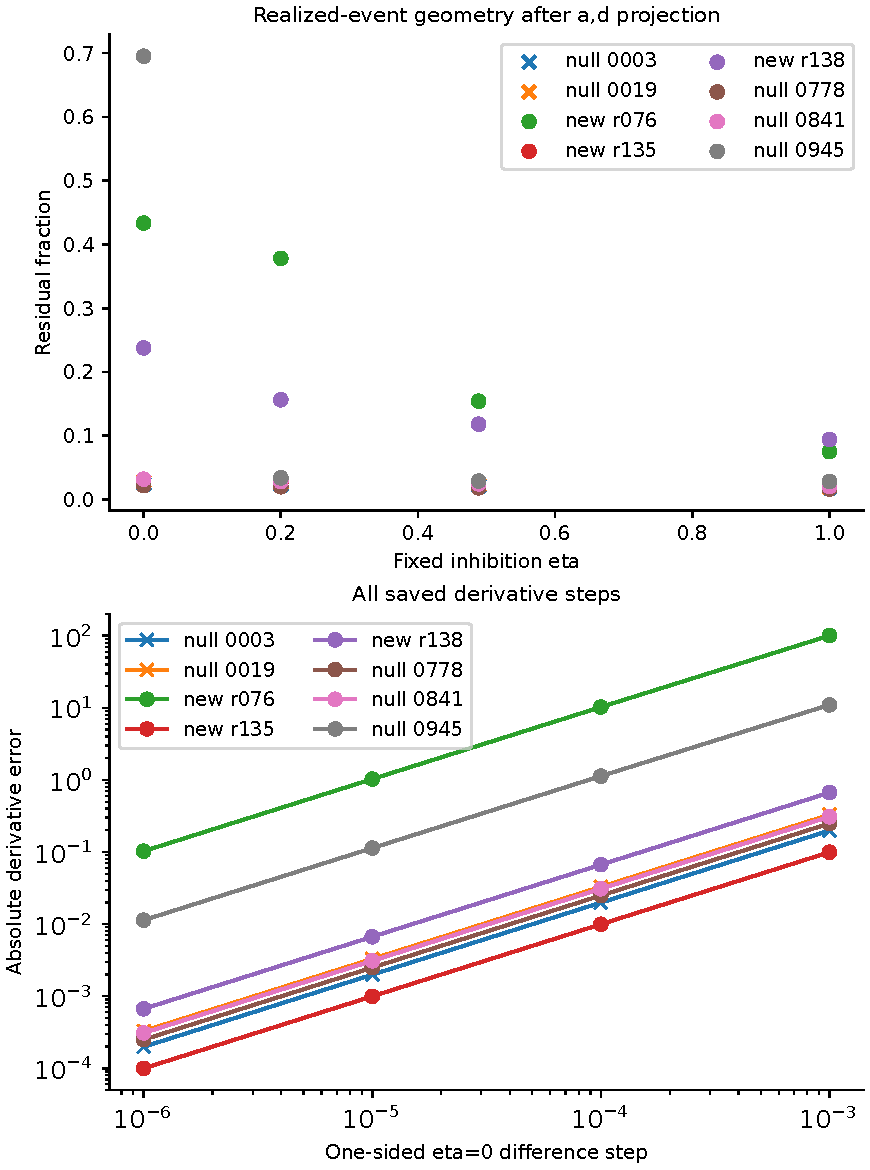
\includegraphics[width=\linewidth,height=.80\textheight,keepaspectratio]{a1_geometry_and_derivative_steps.pdf}
\caption{Realized-event overlap and all saved $\eta=0$ derivative steps.
Positive absolute errors use a log display; exact zeros, if any, are listed
separately without floors, clipping or imputation. Selected old witnesses
remain distinct. Neither panel establishes a causal mechanism.}
\end{figure}

\section{Calibration and uncertainty contract}
Let $R$ be the planned reference count, $K$ the controlled reference indices,
$U=R-|K|$, and $B_q=\sum_{r\in K}\mathbf 1\{T_r\geq T_q\}$ for a controlled
query statistic. The add-one rank interval is
\[
 p_q\in\left[\frac{1+B_q}{R+1},\frac{1+B_q+U}{R+1}\right].
\]
Ties use $\geq$. An uncontrolled query remains unknown. An upper endpoint
at most $\alpha$ gives a definite rejection; a lower endpoint above $\alpha$
gives a definite non-rejection; otherwise the decision remains unknown.
For $N$ planned queries, $k$ definite rejections and $u$ unknowns give
accounting bounds $[k/N,(k+u)/N]$, not sampling confidence intervals.

For the paired nuisance interaction,
\[
 D_i=I_i^{00}-I_i^{10}-I_i^{01}+I_i^{11},\qquad
 \overline D=N^{-1}\sum_iD_i,\qquad
 \operatorname{MCSE}=\sqrt{\frac{\sum_i(D_i-\overline D)^2}{N(N-1)}} .
\]
The declared point summary requires all planned paired rows resolved and
$N\geq2$; it is conditional on the fixed reference bank, not a survivor-only
estimate or reference-bank uncertainty measure.

The executed method used 2,000 shared-reference and paired-query resamples
as a separately gated descriptive sensitivity analysis, not automatic
confirmatory, simultaneous or unconditional coverage. Historical independence
is source-reported, and adaptive pilot/cost-query reuse remains relevant.
Both production jobs ended before final calibration. Independent review
reconstructed base decisions, replayed all 2,000 shared-reference plans and
checked all 80 chunk hashes. It independently recalculated eight declared
query-replicate witnesses.
A separate audit checked all 120 saved endpoint quantiles. This does not mean
every resampled query statistic was independently recalculated.

% Values retained from the independently audited saved-output checkpoint.
\section{Historical bounded checkpoint}
The historical checkpoint inventory retained 2,149 histories: 999 references, 1,000 null
queries and 150 alternative queries. Of 8,596 planned method outcomes,
7,068 have controlled statistics and 1,528 remain unknown. There are 1,752
histories with all four controlled, 18 partial, three with exceptions and
376 never attempted. One of the partial claimed histories was interrupted with
an uncontrolled final method. Registration is not complete computation.
The two production phases produced 1,639 new terminal records and reused
133 immutable carried records; the claim count was 1,640.

At $\alpha=0.05$, the historical checkpoint accounting was:
\begin{center}
\captionof*{table}{Historical incomplete F-continuation decisions and planned-denominator rejection bounds.}
\begin{tabular}{llrrrr}\toprule
Queries & Cell & Reject & Non-reject & Unknown & Rejection bounds\\\midrule
Null ($N=1000$)&$I_{00}$&30&593&377&$[0.030,0.407]$\\
&$I_{10}$&35&588&377&$[0.035,0.412]$\\
&$I_{01}$&31&586&383&$[0.031,0.414]$\\
&$I_{11}$&31&589&380&$[0.031,0.411]$\\\midrule
Alternative ($N=150$)&$I_{00}$&150&0&0&$[1,1]$\\
&$I_{10}$&122&28&0&$[0.8133,0.8133]$\\
&$I_{01}$&150&0&0&$[1,1]$\\
&$I_{11}$&65&82&3&$[0.4333,0.4533]$\\\bottomrule
\end{tabular}
\end{center}
The finite fitting recipe reported here gives 122 rejections out of 150
for $I_{10}$ and 65 rejections, 82 non-rejections and three unknown decisions
for $I_{11}$. These are distinct from the paper's historical counts of
123/150 and 68/150, respectively. A separate source-reported metadata check
matched historical and continuation input identities and case roles; this
compact packet does not reproduce it. No paired historical/continuation
outcome comparison is reported; the counts should not be combined or
interpreted as a paired change in detection.

These are bounds over all planned queries, not confidence intervals or
estimates conditional on successful fitting. Controlled reference counts
are 998, 998, 992 and 997 in cell order; controlled null-query counts are
623, 623, 619 and 620; alternative counts are 150, 150, 150 and 148.
Thus a controlled query can still have an unresolved decision because
reference uncertainty straddles the threshold. Null missingness depends
on history cost, traversal and deadlines; the broad bounds do not establish
empirical 5\% size.

At that checkpoint, the unresolved fraction was too large to establish a useful empirical Type I error rate near the nominal five percent level. Missingness cannot be treated as random: expensive histories, the traversal order and computational limits affect which results resolve. Neither a successful subset nor that checkpoint's resampling repaired the missing null coverage; the completed recovery later in this chapter does so explicitly.

The nuisance-interaction accounting bounds are $[-0.765,0.752]$ under
the null and $[-0.38,-0.36]$ under the alternative. The required full-pair
point mean and MCSE are unavailable for both roles. No survivor-only point
estimate is substituted. On these 150 saved alternative histories, supplying
level and estimating trend gives 150 definite rejections;
estimating both nuisance coordinates is associated with materially fewer
detections. The signed interaction is a procedure contrast, not a causal
effect or proof of physical inhibition.

\subsection{Completed descriptive resampling}
All 2,000 declared replicates completed, using one shared reference plan
across the four cells and both roles, and separate paired query plans by
role. Lower and upper accounting endpoints are summarized separately with
linear/type-7 quantiles. For the alternative $I_{11}$ cell, the 2.5\%, median
and 97.5\% quantiles of the lower endpoint are $(0.3800,0.4333,0.4667)$
for bank-only resampling and $(0.3400,0.4333,0.5200)$ when paired queries
are also resampled. The corresponding upper-endpoint quantiles are
$(0.4067,0.4533,0.4800)$ and $(0.3600,0.4533,0.5400)$.
These summarize sensitivity of incomplete accounting, not certified coverage.
All 120 endpoint quantiles and counts of every replicate status are retained
in the JSON/CSV tables; individual statuses remain in the saved chunk JSON.
No unresolved replicate is discarded. In the alternative
paired-query mode, 126 replicates have a resolved point interaction and
1,874 remain unresolved. This does not resolve the original full-pair point.

\subsection{Posthoc accounting of the continuation pilot}
This subsection concerns the earlier 25-query pilot of this continuation,
not the paper's separate $\eta$-planning experiment (6/25 versus 11/25).
After inspecting the aggregate calibration, a separate saved-evidence check
fixed the original 25 alternative IDs and compared their unchanged carried
scores under the old and expanded reference banks. This was descriptive
posthoc accounting: no fit, rank plan or history was regenerated.
For $I_{10}$, the original cohort changed from $(6,11,8)$ to $(19,6,0)$
in reject/non-reject/unknown counts. The remaining 125 alternatives gave
$(103,22,0)$ under the same final bank. For $I_{11}$, the original cohort
changed from $(6,17,2)$ to $(8,17,0)$ and the remaining cohort gave
$(57,65,3)$. Both cohorts have all rejections in $I_{00}$ and $I_{01}$.
The same 25 fitted scores yield different decisions under the new reference
calibration. This comparison does not isolate bank size from reference
composition, rank resolution or missingness. Neither
this comparison nor the additional query cohort establishes population
causality, independent validation or nominal test size.

\begin{figure}[htbp]
\centering
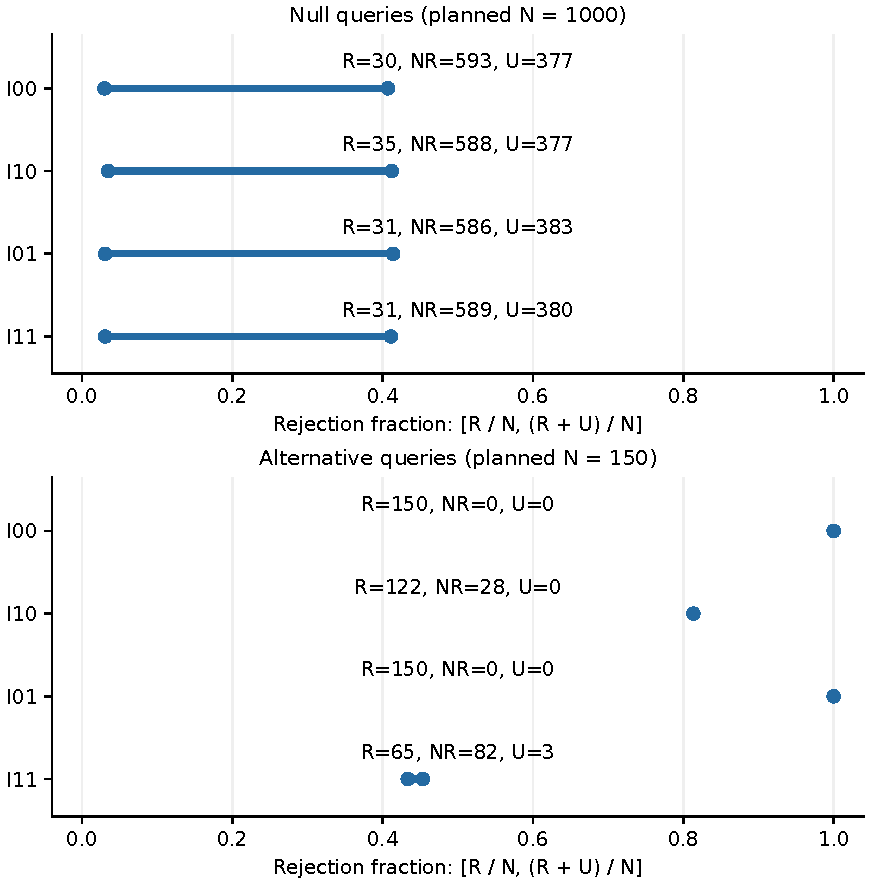
\includegraphics[width=\textwidth]{a1_planned_denominator_bounds.pdf}
\caption*{Historical incomplete calibration on the full planned denominators.
Segments span definite rejection through rejection plus unresolved outcomes;
they are accounting bounds, not confidence intervals. Counts distinguish
definite rejection (R), nonrejection (NR) and unresolved outcomes (U);
reference-bank counts remain in the accompanying text.}
\end{figure}

\begin{figure}[htbp]\centering
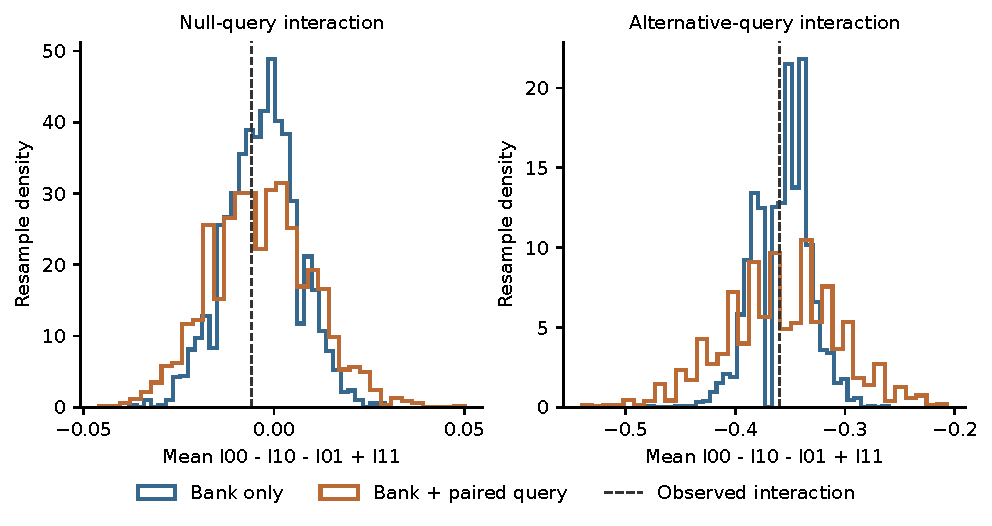
\includegraphics[width=\textwidth]{s01_saved_bootstrap_interactions.pdf}
\caption{The saved 2,000 resampled interaction means for each role and mode.
No additional fit or resampling was performed to draw this figure.}
\end{figure}

\subsection{Decision at the historical checkpoint}
The earlier continuation stopped incomplete and called for a cheaper, numerically validated recovery. The completed missing-only recovery below now supplies resolved counts; it preserves old failures as history and recalculates the rank decisions against the repaired reference bank.

\section{Availability and bounded interpretation}
The 2,149 reused bank byte/clock identities were reverified; the historical
RNG and generating process were not replayed at that checkpoint. The original
source-only delivery omitted the NPZ bank; the recovered-input edition now
supplies its exact histories and role, seed and clock mapping under
\path{reproduction/synthetic/}. Some original F restricted-fit states remain
missing and are not replaced by unrelated earlier fit records.
The accompanying saved summary, accounting tables and figures document the
reported numerical checkpoint; they do not replace the raw-history replay.
The saved \texttt{F\_RESULT\_TABLES.json} records an input
\texttt{summary.json} SHA-256 beginning \texttt{456a3c1f}, whereas
the bundled summary has SHA-256 beginning \texttt{32115580}.
The matrix counts and all displayed endpoint quantiles agree under
saved-value reconciliation; that agreement does not establish byte-identical
input provenance.

Conditional overlap, solver flags and controlled calibration outcomes must be
interpreted together with failures and missing tails. They do not identify
physical inhibition or justify an automatic cache change, retry, new bank,
broader search or next cycle. The separately authorized recovery below addresses that proposal; it retains the predictive and causal interpretation limits.

\subsection{Historical endpoint sensitivity and unresolved interactions}
All endpoint quantiles remain in Appendix~\ref{app:f-endpoints}, Table~\ref{tab:f-all-endpoints}. The repeated point-interaction statuses reduce to the four rows below. The 2,000 resamples per role and mode produced accounting-bound endpoints; an unresolved point interaction does not mean that its endpoint calculation failed. Repeating a status across ten endpoint rows does not create ten new resampling cohorts.
\begin{center}
\begin{tabular}{llrr}\toprule
Role & Resampling & Resolved & Unknown\\\midrule
Null & Bank only & 0 & 2000\\
Null & Bank and paired query & 0 & 2000\\
Alternative & Bank only & 0 & 2000\\
Alternative & Bank and paired query & 126 & 1874\\\bottomrule
\end{tabular}
\end{center}
These are descriptive sensitivity calculations, not confidence limits. Even a resolved resampled point does not resolve the original full-pair statistic or establish null calibration.

% Source: M01/S01_SUMMARY.json SHA256 b04416906237b7dfbaf8af5ef8f08b7e9147d10155e495bfcc9a694a5bb691a8.
% Acceptance: scientific_stage2_resume_20261031T205913Z/integration/S01_ACCEPTANCE.json.
% Figures and complete input bindings: temporal/integration/source_bindings.json.
\section{Completed F-continuation recovery}
The earlier incomplete continuation is a historical checkpoint, rather than
the final coverage statement. The authorized Stage~2 recovery filled only
missing statistics: 11 reference histories, 384 null-query histories and two
alternative-query histories, comprising 397 histories and 1,528 procedure
cells. The earlier shorthand of 383 null and three alternative histories is
superseded by this bound input map. All 7,068 originally controlled cells
were preserved. The final bank contains 999 reference statistics, 1,000 null
queries and 150 alternative queries for each of $I_{00},I_{10},I_{01},I_{11}$,
with no unresolved cells. Calibration uses the same add-one rank rule,
including ties through reference statistics greater than or equal to the
query statistic.

\begin{table}[htbp]\centering
\caption{Completed F-continuation rejection counts. All planned queries are
resolved; these proportions replace the historical missingness bounds as
the current numerical checkpoint.}\label{tab:f-stage2-completed}\label{tab:f-continuation}
\begin{tabular}{lrrrr}\toprule
Queries & $I_{00}$ & $I_{10}$ & $I_{01}$ & $I_{11}$\\\midrule
Null ($N=1{,}000$) & 49 (0.049) & 47 (0.047) & 52 (0.052) & 44 (0.044)\\
Alternative ($N=150$) & 150 (1.000) & 122 (0.8133) & 150 (1.000) & 68 (0.4533)\\\bottomrule
\end{tabular}\end{table}

\begin{table}[htbp]\centering
\caption{Completed recovery coverage. Query counts apply to each of the four procedures; repaired and preserved counts refer to procedure cells.}\label{tab:f-recovery-coverage}
\begin{tabular}{lr}\toprule
Quantity & Completed count\\\midrule
Reference histories per procedure & 999\\
Null queries per procedure & 1,000\\
Alternative queries per procedure & 150\\
Preserved procedure cells & 7,068\\
Repaired missing procedure cells & 1,528\\
Profile meshes & 11 of 11\\\bottomrule
\end{tabular}\end{table}

The completed paired interaction
$\overline D=\overline{I^{00}-I^{10}-I^{01}+I^{11}}$ is $-0.006$ under
the null queries (query-unit Monte Carlo standard error $0.00949$), and
$-0.360$ under the alternatives (standard error $0.04564$).
The 2,000 saved resamples in each role and resampling mode are all resolved.
\begin{table}[htbp]\centering
\caption{Completed paired nuisance-interaction means and query-unit Monte Carlo standard errors.}\label{tab:f-completed-interaction}
\begin{tabular}{lrr}\toprule
Queries & Mean $\overline D$ & Monte Carlo SE\\\midrule
Null ($N=1{,}000$) & $-0.006$ & $0.00949$\\
Alternative ($N=150$) & $-0.360$ & $0.04564$\\\bottomrule
\end{tabular}\end{table}
Their descriptive 2.5th, 50th and 97.5th percentiles appear in Table~\ref{tab:f-completed-bootstrap}.

% Completed Stage 2 bootstrap table; historical endpoints retained separately.
\begin{table}[htbp]\centering
\caption{Completed paired-interaction bootstrap summaries. All 2,000 replicates per row are resolved; quantiles are descriptive resampling summaries.}\label{tab:f-completed-bootstrap}
\begin{tabular}{llrrr}\toprule
Queries & Resampling & 2.5th & 50th & 97.5th\\\midrule
Null & Bank only & $-0.022$ & $-0.003$ & $0.015$\\
Null & Bank and paired query & $-0.029$ & $-0.004$ & $0.023$\\
Alternative & Bank only & $-0.4067$ & $-0.3533$ & $-0.3067$\\
Alternative & Bank and paired query & $-0.4667$ & $-0.3600$ & $-0.2533$\\\bottomrule
\end{tabular}\end{table}


These are reference-bank and paired-query resampling sensitivity summaries,
not certified confidence coverage or an independent population calibration.
The null rates are observed simulation frequencies, not proof of nominal
size for every generating law.

\begin{figure}[htbp]\centering
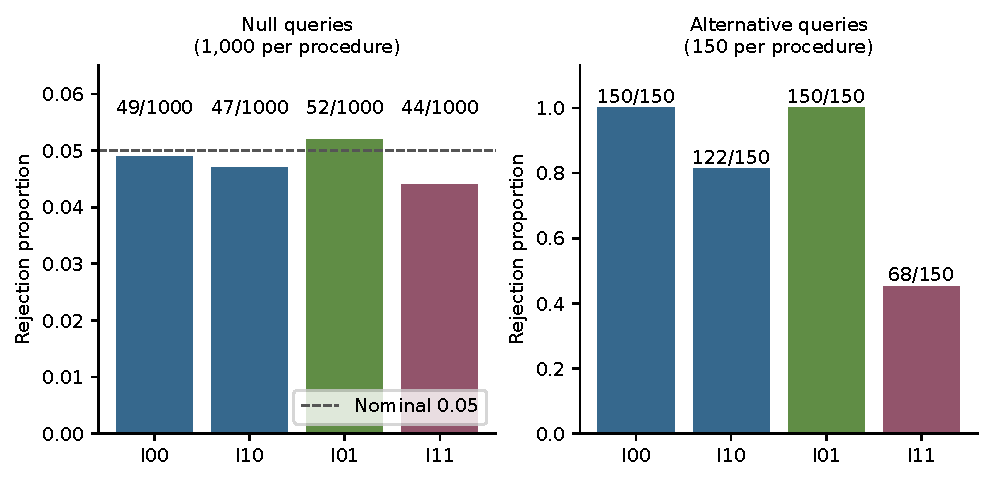
\includegraphics[width=\textwidth]{s01_completed_rejections.pdf}
\caption{Completed planned-denominator F-continuation rejection proportions.
No unresolved outcomes are imputed. The dashed line denotes nominal 0.05.}
\end{figure}



The reference-bank calibration remains an oracle calibration for the
specified synthetic law. It is not a nested fitted-null plug-in calibration:
the proposed 23,760-fit nested bootstrap was excluded by the authorized
scope. Recovery combines original controlled results with an eight-start
compiled procedure only for missing cells, and therefore does not claim
uniform reoptimization of every bank member. Validation comprises 20
resolved-history compatibility controls, independent kernel fixtures and a
three-history raw saved-point pilot, together with complete saved custody
and aggregate arithmetic checks. It does not claim independent raw replay
of every fit or mesh. The finite 195-mode approximation and predictable
pre-event clock convention remain those of the preserved implementation.

